\documentclass[a4paper,onecolumn,10pt]{article}
\usepackage[polish]{babel}
\usepackage[utf8]{inputenc}
\usepackage[T1]{fontenc}
\usepackage[left=2.1cm,right=2.1cm]{geometry}
\usepackage[dvipsnames]{xcolor}
\usepackage{amsmath,calc,indentfirst,fancyhdr,amsfonts,graphicx,epstopdf,caption, mathcomp, subcaption,wrapfig, siunitx,pbox,float,algorithm}
\usepackage[noend]{algpseudocode}


\makeatletter
\def\BState{\State\hskip-\ALG@thistlm}
\renewcommand{\ALG@name}{Algorytm}
\makeatother

\renewcommand{\baselinestretch}{1.1}	 % odstep miedzy liniami
\addto\captionspolish{\renewcommand{\figurename}{Wykres}} % zmiana podpisu pod obrazkami, zamiast "Rysunek" bedzie "Wykres"
\newcommand{\NN}{\mathbb{N}}			 % makro do znaku liczb naturalnych

\newcommand{\R}[1]{\textcolor{red}{#1}}  % makro do polecenia z parametrami - tutaj 1 parametr
\newcommand{\G}[1]{\textcolor{green}{#1}} 
\newcommand{\B}[1]{\textcolor{RoyalBlue}{#1}} 
% kolorowanie {\B{argument}}

\newcommand{\PICTURES}{} % szybsza kompilacja dzieki stalej "usuwajacej" obrazki
						 % zakomentowanie \PICTURES powoduje znikniecie obrazkow

\pagestyle{fancy} % formatuj caly dokument
\fancyhead{}
\fancyfoot{}
\renewcommand{\headrulewidth}{0pt}
\fancyfoot[R]{\thepage} % dla stron poza tytulowa nr w prawym dolnym rogu

\fancypagestyle{plain}{ % dla strony tytulowej nr w prawym dolnym rogu
	
	\renewcommand{\headrulewidth}{0pt}
	\fancyhf{}
	\fancyfoot[R]{\thepage}
}
% 17 linia w preamble.tex

\renewcommand{\arraystretch}{1.2}

\title{\Large\vspace{-2.5cm}{\Huge S}PRAWOZDANIE - LABORATORIUM NR {\Huge10}\\
	\textbf{Poszukiwanie minimum wartości funkcji\\ metodą największego spadku w 2D} } 
\date{\Large16 maja 2019}
\author{\Large Marek Kiełtyka}

\begin{document}
\maketitle

\vspace{-1.2cm}\section{Wstęp}

\subsection{Minimalizacja funkcji}
Inaczej nazywana optymalizacją, jej zadaniem jest poszukiwanie odpowiednio minimum lub maksimum funkcji wielu zmiennych. Chodzi o znalezienie punktu spełniającego warunek
\begin{equation}
\min f(\vec{x}) = f(\vec{x^{*}}) \Leftrightarrow \bigwedge_{\vec{x} \in R^n} f(\vec{x^{*}}) < f(\vec{x}), \quad \text{ gdzie } \vec{x} = [x_1, x_2, \dots, x_n]^{T}.
\end{equation}
\subsection{Gradient funkcji}
Dla funkcji celu $f(\vec{x}) \in C^2$, tj. poszukującej minimum badanej funkcji wejściowej definiuje się funkcję wektorową będącą gradientem funkcji
\begin{equation}
g(\vec{x}) = \nabla f(\vec{x}) = \bigg[ \frac{\partial f(\vec{x})}{\partial x_1}, \frac{\partial f(\vec{x})}{\partial x_2}, \dots, \frac{\partial f(\vec{x})}{\partial x_n}, \bigg]^{T}.
\end{equation}
Należy pamiętać, iż gradient skierowany jest zawsze w stronę narastających wartości.
\subsection{Pochodna kierunkowa funkcji celu}
Różniczkę zupełną funkcji celu definiuje się jako iloczyn skalarny wektorów
\begin{equation}
df = \frac{\partial f}{\partial x_1} dx_1 +  \cdots + \frac{\partial f}{\partial x_n} dx_n = \nabla f(\vec{x}) dx.
\end{equation}
Punkty  $\vec{x}$ i $\vec{x'}$ nazywane są powiązanymi ze sobą, jeżeli wektor $\vec{u}$ wyznacza kierunek prostej je łączącej, stąd
\begin{equation}
\vec{x}(\lambda) = \vec{x'} + \lambda \vec{u} .
\label{lambda}
\end{equation}
Dla bardzo małych zmian wartości $\lambda$ można uogólnić wzór (\ref{lambda}).
\begin{equation}
d\vec{x} = \vec{u} d\lambda
\end{equation}
Na prostej łączacej ustalone punkty $\vec{x}$ oraz $\vec{x'}$ wartość funkcji celu zależna jest od zmiennej $\lambda$.
\begin{equation}
F(\lambda) = f(\vec{x'} + \lambda \vec{u} ) = f(\vec{x})
\end{equation}
Mając na uwadze powyższe powiązania, oblicza się różniczkę zupełną dla funkcji celu zależnej od $\lambda$
\begin{equation}
dF = df = \nabla^{T} f(\vec{x}) \vec{u} d \lambda.
\end{equation}
Finalnie, wyrażenie na \textbf{pochodną kierunkową funkcji} celu w punkcie $\vec{x}$ dla kierunku $\vec{u}$ jest postaci
\begin{equation}
\frac{d F (\lambda)}{d\lambda} = \left.\frac{df(\vec{x})}{d\lambda}\right|_{\vec{u}} = \nabla^{T} f(\vec{x}) \vec{u}, 
\label{wzor}
\end{equation}
jednak korzystając z niej należy ją wyznaczać w każdej iteracji.

\subsection{Znajdowanie minimum funkcji przy pomocy pochodnej kierunkowej}
Przybliżanie należy rozpocząć z punktu $\vec{x_0}$ przechodząc przez kolejne punkty $\vec{x_1}, \vec{x_2}, \dots, \vec{x_n}$ w kierunku spadku wartości funkcji. Pozwala to wyznaczyć ciąg przybliżeń poszukiwanego minimum. Należy przerwać algorytm iteracyjny w momencie, gdy zostanie spełniony jeden z warunków:
\begin{enumerate}
	\item Norma różnicy wektorów z sąsiednich kroków jest mniejsza od zadanego progu: $||\vec{x}^{i+1} - \vec{x}^i|| < \epsilon$
	\item $\nabla f(\vec{x}) = 0$
	\item W kolejnych iteracjach wartość normy $||\vec{x}^{i+1} - \vec{x}^i||$ wzrasta, co oznacza brak zbieżności.
\end{enumerate}
\subsection{Metoda największego spadku}
Wykorzystuje się\begin{itemize}
	\item wzór (\ref{wzor}) w punkcie $\vec{x'}$ dla wektora kierunkowego $\vec{u}$ o długości równej $||\vec{u}|| = 1$
	\begin{equation}
	\left.\frac{\text{d}f(\vec{x'})}{\text{d}\lambda}\right|_{\vec{u}} = \frac{\text{d}F(0)}{\text{d}\lambda} = 
	\nabla ^{T} f(\vec{x'})\vec{u},
	\end{equation}
	\item nierówność Schwartza \begin{equation}
	\nabla^{T} f(\vec{x'}) \vec{u} \geq - ||\nabla^{T} f(\vec{x'})|| \cdot || \vec{u}  || = 
	- || \nabla ^{T} f(\vec{x'})|| = \min.
	\end{equation}
\end{itemize} 
Należy wybrać wektor kierunkowy o postaci
\begin{equation}
\vec{u} = \frac{- \nabla f(\vec{x'})}{||\nabla f(\vec{x'})||}
\end{equation}
aby wskazywał kierunek największego spadku, a pochodna kierunkowa mogła osiągnąć najmniejszą wartość.
\begin{equation}
\frac{\text{d} F(0) }{\text{d} \lambda} = - \nabla^T f(\vec{x'})  \frac{\nabla f(\vec{x'})}{||\nabla f(\vec{x'})||} = \min
\end{equation}

\newpage
\section{Zadanie do wykonania}

\subsection{Opis problemu}

Celem laboratorium było znalezienie minimum zadanej funkcji (\ref{lol}) przy pomocy opisywanej metody
\begin{equation}
f(\vec{r}) =  f(x, y) = \frac{5}{2} (x^2 - y)^2 + (1 - x )^2,
\label{lol}
\end{equation}
począwszy od przybliżenia $\vec{r_0}$ postaci
\begin{equation}
\vec{r_{i+1}} = \vec{r_i} - h\cdot\nabla \left.f(\vec{r})\right|_{\vec{r} = \vec{r_i}} \quad \text{ gdzie } \nabla f(\vec{r}) = \left[\frac{\partial f}{\partial x}, \frac{\partial f}{\partial y}\right],
\label{15}
\end{equation}
które było korygowane w kolejnych iteracjach.
Składowe gradientu ze wzoru (\ref{15}) obliczano numerycznie korzystając z faktu, iż
\begin{equation}
\frac{\partial f(x_i,y_i)}{\partial  x} \approx \frac{f(x_i + \Delta x, y_i) - f(x_i - \Delta x, y_i)}{2 \Delta x}
\end{equation}
\begin{equation}
\frac{\partial f(x_i,y_i)}{\partial y} \approx \frac{f(x_i, y_i  + \Delta y) - f(x_i, y_i - \Delta y)}{2 \Delta y}
\end{equation}
Przyjęto następujące założenia:
\begin{itemize}
	\item punkt początkowy $\vec{r_0} = [-0.75, 1.75]$
	\item stała $h = 0.01$
	\item warunki stopu \begin{itemize}
		\item $||\vec{r_{i+1}} - \vec{r_i}||_2 < \epsilon$ dla $\epsilon_1 = 10^{-2}$, $\epsilon_2 = 10^{-3}$
		\item maksymalna liczba iteracji \textit{maxIter} $ = 1000 $
	\end{itemize}
	\item $\Delta x = \Delta y = \Delta = 10^{-4}$
	\item  $x, y \in [-2, 2]$ z krokiem w obu kierunkach równym 0.02
\end{itemize}


\newpage
\subsection{Wyniki}

Korzystając z programu napisanego w języku C++ i spreparowanego wcześniej skryptu programu \textit{Gnuplot} sporządzono wykresy dla obu przypadków. Rozważano jedną funkcję, zatem dokładne jej minimum było jedno i wyniosło $ x_{min} = 1, y_{min} = 1 $.
\begin{figure}[h!]
	\begin{center}
		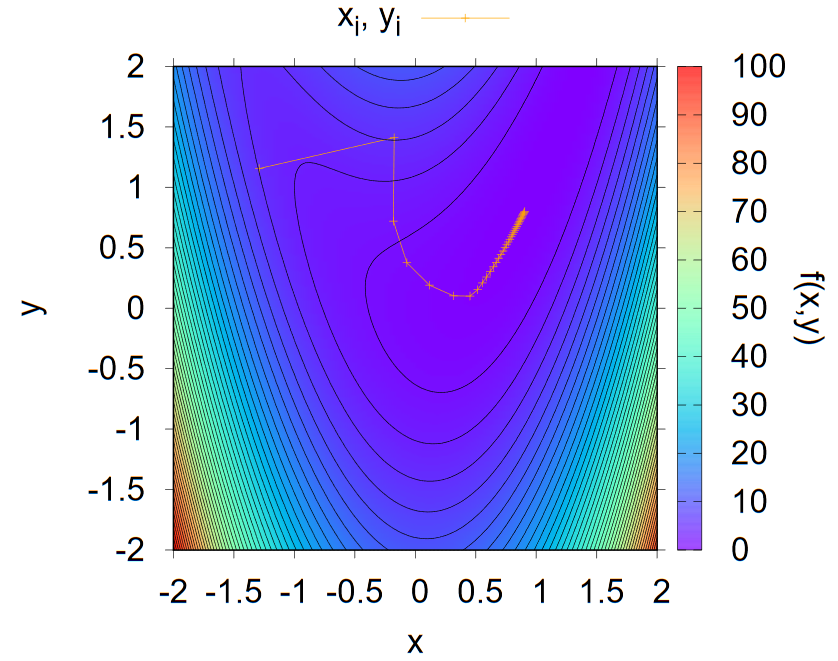
\includegraphics[height=0.41\linewidth]{min1.png}
	\caption{Położenia kolejnych przybliżeń minimum funkcji $ f(x, y) $ w poszczególnych iteracjach dla $\epsilon = 10^{-2} $. W tle: kontury oraz mapa wartości funkcji $ f(x, y) $. Program wykonał 37 iteracji.}
	\label{pierwszy} 
	\end{center}
\end{figure}
\begin{figure}[h!]
	\begin{center}
	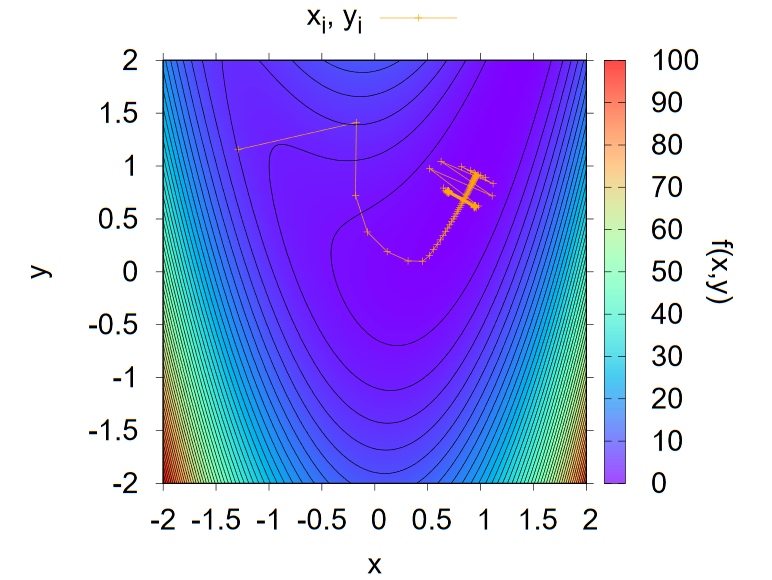
\includegraphics[height=0.41\linewidth]{min2.png}
	\caption{Położenia kolejnych przybliżeń minimum funkcji $ f(x, y) $ w poszczególnych iteracjach dla $\epsilon = 10^{-3} $. W tle: kontury oraz mapa wartości funkcji $ f(x, y) $. Program wykonał 1000 iteracji.}
	\label{drugi} 
\end{center}
\end{figure}

\newpage
\section{Wnioski}

Wykresy dowodzą, iż ciężko jest wybrać trafne kryterium zbieżności. Dla pierwszego przypadku nie udało się osiągnąć minimum, choć przebieg ($x_i, y_i$) zdawał się być na dobrej drodze ku temu. Zmniejszając rząd zbieżności o jeden, zastosowanie znalazł drugi warunek stopu z uwagi na niekończące się oscylacje wokół poszukiwanego minimum. Potwiedziło to również teoretyczny kształt przebiegu ($x_i, y_i$) dla funkcji z wydłużonym konturem.

Jedynym parametrem, który można by zmodyfikować dla lepszej efektywności obliczeń, jest $h$. Z racji jego stałości podczas laboratorium skoki nie były regulowane, co znalazło szczególne odbicie w punktach funkcji o\,niewielkim gradiencie, a w konsekwencji nie osiągnięto zbieżności.

Mimo tych niedoskonałości, metoda największego spadku prowadzi do znalezienia minimum funkcji wielu zmiennych w sposób szybki i prosty.
\end{document}